\chapter{Einleitung}

%----------------------------------------------------------------------------------------

Die folgenden Kapitel beschreiben den Prozess, der nötig war um das Schloss
Rapperswil mittels Luftbilder als 3D-Modell zu rekonstruieren. Wir gehen hier
nicht auf die Evaluation der genutzten Software ein, dies folgt im nächsten Teil
dieser Dokumentation.

%----------------------------------------------------------------------------------------

\section{Erfassung des Schlosses mit Kamera-Drohne}

Um Fotos des Schlosses von allen Winkeln zu erstellen, braucht man ein
ferngesteuertes Flugobjekt wie z.~B. einen Multikopter. In unserem Fall wurden
die Fotos von Michael Suter (\url{http://lightmoment.ch/}) erstellt, der einen
Quadrokopter besitzt und daran freundlicherweise seine Piloten-Fähigkeiten unter
Beweis gestellt hat.

\subsection{Materialliste}

\begin{itemize}
	\item Quadrokopter: \textit{Team BlackSheep Discovery
		Pro}\footnote{\url{http://www.team-blacksheep.com/products/prod:discopro}}
	\item Kamera: \textit{GoPro Hero 4 Black}\footnote{\url{https://gopro.com/}}
	\item GPS Tracker: \textit{Fairphone
		FP1}\footnote{\url{https://www.fairphone.com/}} mit
		\textit{GeoTracker}
		App\footnote{\url{https://play.google.com/store/apps/details?id=com.ilyabogdanovich.geotracker}}
\end{itemize}

\subsection{Vorgehen}

Die maximale Flugzeit pro Akku beträgt 10--15 Minuten. Wir hatten 2 geladene
Akkus dabei und erreichten somit eine Flugzeit von 20--30 Minuten.

Die GoPro Kamera hatten wir so eingestellt, dass sie zwei mal pro Sekunde ein
Bild machte. Daraus ergaben sich dann etwa 2700 Fotos, was ca. 5.3 GiB
Bildmaterial entspricht.

Um die GPS-Koordinaten aufzuzeichnen, haben wir ein Smartphone mit einer GPS
Tracking App auf dem Quadrokopter befestigt. Das ist nicht sehr professionell,
hat aber gut funktioniert.

\begin{figure}[p]
	\centering
	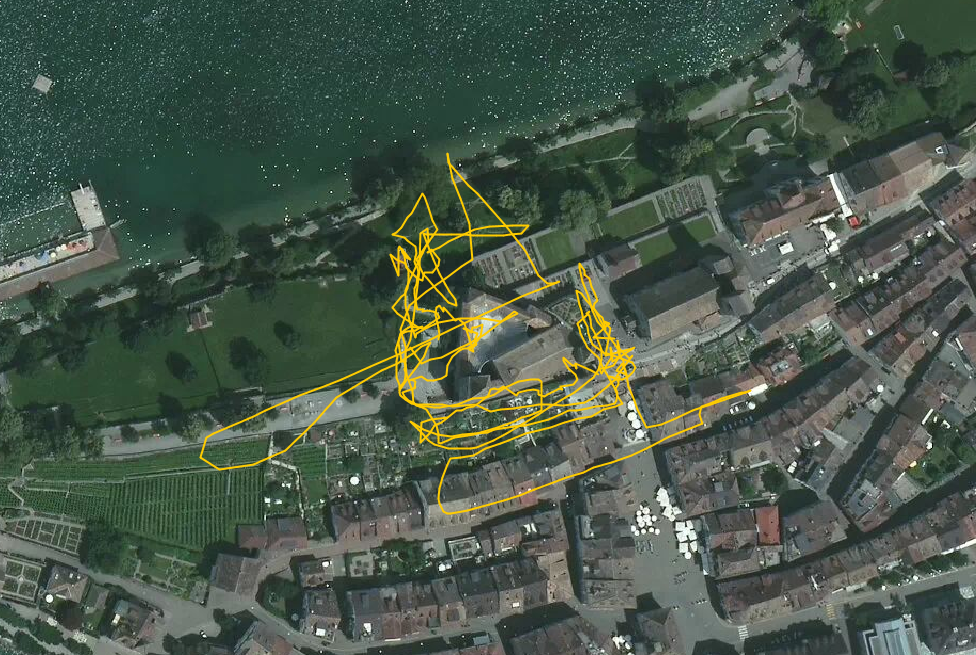
\includegraphics[width=\textwidth]{images/gpstrace_satellite.png}
	\caption{GPS Trace des Quadrokopters während der Erfassung.\\Bildmaterial:
		\copyright{} Bing Maps}
	\label{img:gpstrace-satellite}
\end{figure}

\begin{figure}[p]
	\centering
	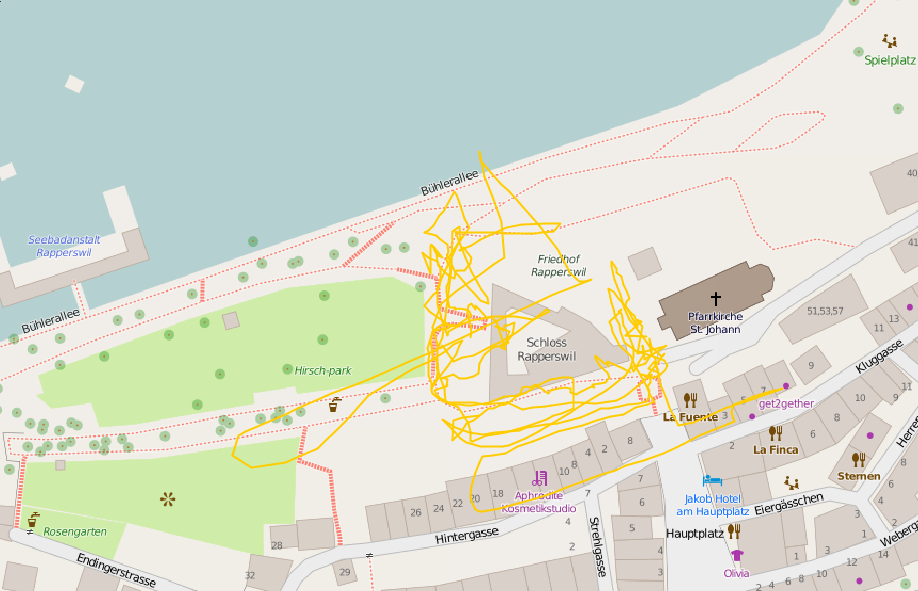
\includegraphics[width=\textwidth]{images/gpstrace_mapnik.png}
	\caption{GPS Trace des Quadrokopters während der Erfassung.\\Bildmaterial:
		\copyright{} OpenStreetMap Contributors}
	\label{img:gpstrace-mapnik}
\end{figure}
